\documentclass[25pt]{tikzposter}
\usepackage[sfdefault]{FiraSans}
\usepackage{bm}
\usepackage{amsfonts}       % blackboard math symbols
\usepackage{amsmath}

\geometry{paperwidth=90cm, paperheight=122cm}

% metropolis colors
\definecolor{mDarkTeal}{HTML}{23373b}
\definecolor{mDarkBrown}{HTML}{604c38}
\definecolor{mLightBrown}{HTML}{EB811B}
\definecolor{mLightGreen}{HTML}{14B03D}

\usepackage{tikzposterSDU}
\usetheme{SDU}

% background color
\colorlet{blockbodybgcolor}{white}
\colorlet{backgroundcolor}{mDarkTeal}

% custom commands
\newcommand{\half}{\frac{1}{2}}
\newcommand{\x}{\bm{x}}
\newcommand{\xh}{\hat{\bm{x}}}
\newcommand{\e}{\bm{e}}
\newcommand{\z}{\bm{z}}
\newcommand{\mz}{\bm{\mu}_{z}}
\newcommand{\w}{\bm{w}}
\newcommand{\bo}{\bm{b}}
\newcommand{\A}{\bm{A}}

\newcommand{\se}{\sigma_e}
\newcommand{\sz}{\bm{\sigma_z}}
\newcommand{\laz}{\bm{\lambda}_z}

\newcommand{\X}{\bm{X}}
\newcommand{\Z}{\bm{Z}}
\newcommand{\N}{\mathcal{N}}
\newcommand{\U}{\mathcal{U}}
\newcommand{\E}[2]{\text{E}_{#1}\left[#2\right]}
\newcommand{\KL}{\text{KL}}


\begin{document}
% remove offset that would otherwise be fixed by \maketitle
\makeatletter
    \setlength{\TP@blocktop}{.47\textheight}
\makeatother

\colorlet{blockbodybgcolor}{mDarkTeal}
\block{}{
  \color{white}{
    \fontseries{l}\fontsize{130}{100}\selectfont
    Learning \textbf{physical concepts}  purely \\\\\\
    from data: We demonstrate how \\\\\\
    \textbf{generative models} can learn  \\\\\\
    \textbf{manifolds} of \textbf{differential equations.}
  }
}
\colorlet{blockbodybgcolor}{white}


\begin{columns}
  \column{0.7}
  \block{}{
    {\Huge\bf Rodent: Relevance determination in ODE \\\\}
    {\Large Niklas Heim, V\'aclav \v Sm\'idl, Tom\'a\v s Pevn\'y} \hfill
    {\Large Czech Technical University, Prague}
  }

  \block{}{
    \begin{center}
    {\huge\bf Learning differential equations}
    \end{center}
    \begin{minipage}{.28\textwidth}
      \innerblock{}{
      \begin{itemize}
        \item We want to find the simplest ODE that describes a dynamical
          system
        \item By simple we mean: minimal order of ODE and minimum number of
          non-zero parameters.
      \end{itemize}
      }
    \end{minipage}
    \hspace{.02\textwidth}
    \begin{minipage}{.28\textwidth}
      \innerblock{}{
        \begin{itemize}
        \item Discover physically meaningful equations
          that might help understand the underlying process.
        \item We can learn manifolds of generating models not only a single process
          % \item Sparsity enforcing generative model
          % \item ODE solver acts as decoder
          % \item Latent variables are physically interpretable
          % \item Capable of learning ODE manifolds
        \end{itemize}
      }
    \end{minipage}

    \begin{tikzfigure}
      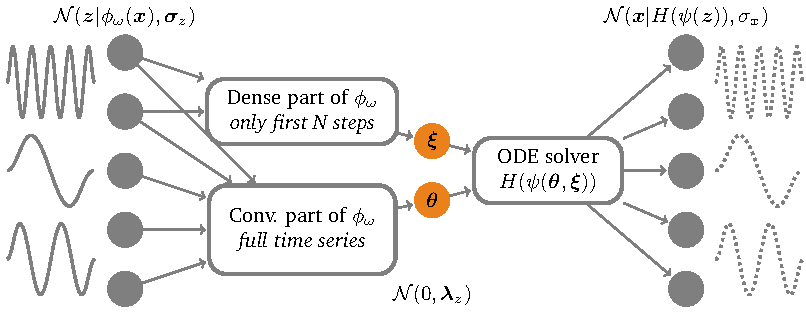
\includegraphics[width=.50\textwidth]{rodent.pdf}
    \end{tikzfigure}

    \vspace{1cm}
    \begin{center}
      {\huge\bf Advantages of the relevant ODE identifier}\\
    \end{center}

    \vspace{1cm}
    \begin{minipage}[t]{.28\textwidth}
    \begin{itemize}
      \item \textbf{Explainability.}  The parameters of $\bm z$ are
        decoded through an ODE solver, which gives them physical meaning.
      \item \textbf{Sparsity.} The automatic relevance determination prior on
        $\bm{z}$ encourages the simplest solution with fewest non-zero parameters.
    \end{itemize}
    \end{minipage}
    \hspace{.01\textwidth}
    \begin{minipage}[t]{.28\textwidth}
    \begin{itemize}
      \item \textbf{Partial observations.} Rodent allows learning of an ODE
        without knowledge of all state trajectories. The
        observation operator is assumed to be known.
      \item \textbf{Time series.} The convolutional part of the encoder is
        agnostic to different time series lengths.
    \end{itemize}
    \end{minipage}


    \vspace{1cm}
    \begin{center}
      {\huge\bf Manifold learning \& Reidentification}\\
    \end{center}
    \begin{tikzfigure}
      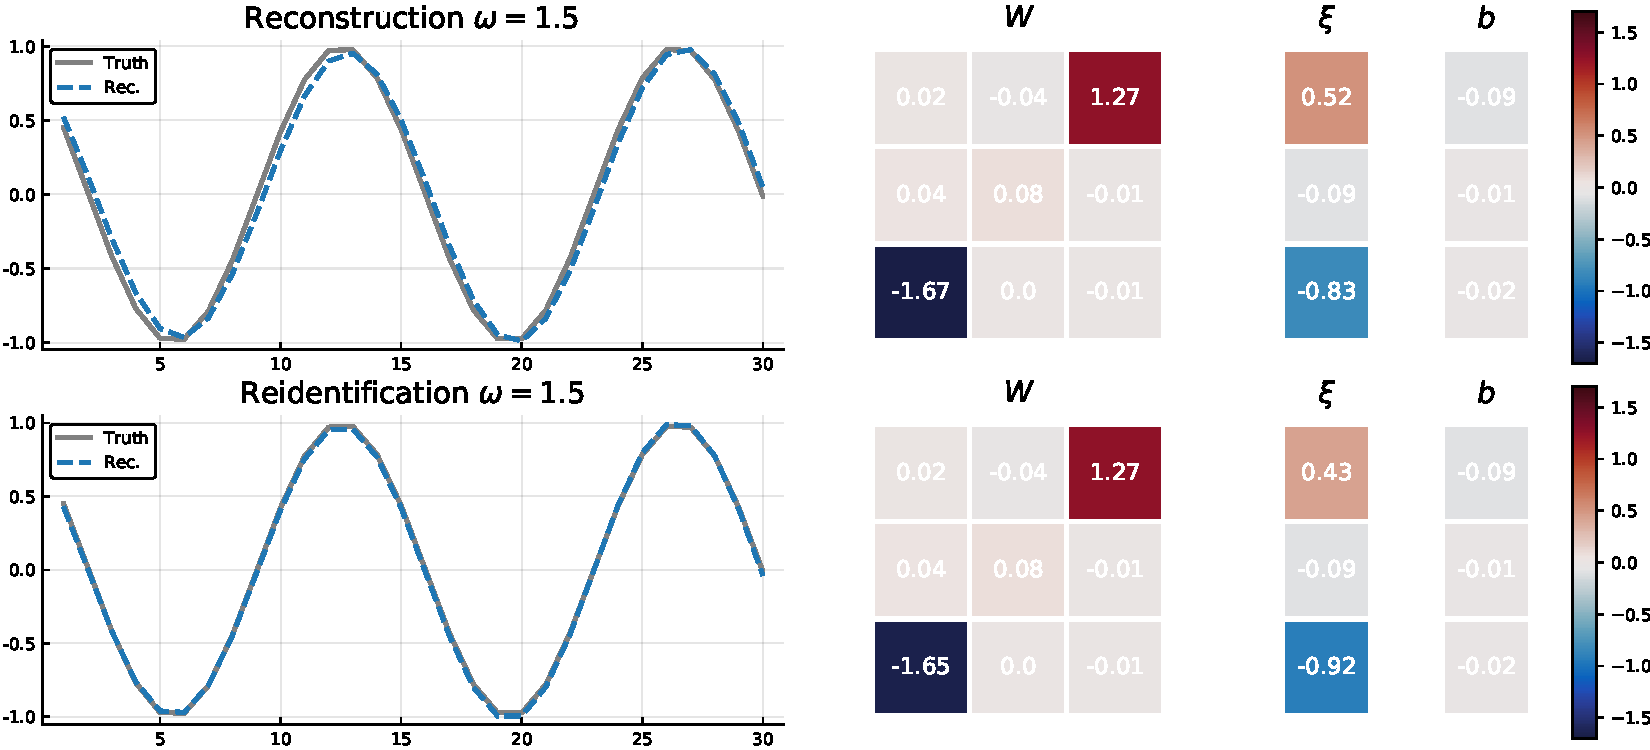
\includegraphics[width=.50\textwidth]{single_enc_rec.pdf}
    \end{tikzfigure}
    Rodent reconstructions (left column) and latent codes (right column) of a
    harmonic signal in the upper plots. Reidentified reconstruction and
    encodings in the bottom.  The values of the latent codes only change were
    the variables were detected as relevant.  The heatmaps on the right show
    the corresponding encodings for the weights $\bm W$, biases $\bm b$, and
    initial conditions $\bm\xi$. The Rodent reduced
    the latent space to the four truly relevant parameters.

  }

  \column{0.3}
  \block{Rodent in depth}{
    Assume a time series $\X = [\bm x_1, \bm x_2,\ldots, \bm x_K]$ with $\bm x_i
    \in \mathbb{R}^d$ generated from discrete-time, noisy observations
    \begin{equation}
      \bm x_k = H(\bm{\xi}(\Delta t k)) + e_k,
    \end{equation}
    where $k=1\ldots K$, $e_k \sim \N(0,\se^2\mathbf{I})$, and partial obs.
    operator $H$.  The evolution of $\bm\xi(t) \in \mathbb{R}^N$ is governed by
    an ODE:
    \begin{align}
      \label{eq:dyn_sys}
      \frac{\partial \bm{\xi}}{\partial t} 
        = & f(\bm{\theta}, t) \approx \bm{W}\bm{\xi} + \bm{b}.
    \end{align}
    We aim to learn structure and order of the ODE from a set of
    trajectories $\{\X_i\}_{i=1}^{L}$  generated by the same generative process
    but with  different $\bm\theta_i$ and different $\bm\xi_i(0)$, for each
    trajectory, i.e.
    \begin{align}
      \label{eq:series_x}
      \X_i =& H(\psi(\bm\theta_i,\bm{\xi}_i(0), \bm{t}))+\bm{e},
    \end{align}
    where $\bm{t} = [0, \Delta t, \ldots, K\Delta t]$ and ODE
    solver $\psi$.  Assuming we observe a system with expected order $M$, we choose $N
    \geq M$.

    If ODE state and parameters are combined in $\z=[\bm\theta,\bm\xi(0)]$ the
    likelihood becomes
    \begin{align}
      \label{eq:decoder}
      p(\x|\z) &= \N(\x|H(\psi(\z)),\sigma_x^2).
    \end{align}
    To determine the structure of the ODE, we employ the ARD prior:
    \begin{align}
      \label{eq:ard_model}
      p(\z) &= \N(\z|0,\text{diag}(\laz^2)) &
      p(\laz) &= 1/\laz.%\Gamma(\laz|\alpha_0, \beta_0)
    \end{align}

    The posterior of $\bm z$ is prescribed by
    \begin{align}
      \label{eq:ard_posterior}
      p(\z|\x) = \N(\z|\phi_\omega(\x), \bm{\sigma}_z^2)
    \end{align}
    where mean $\mz=\phi_\omega(\x)$ is a NN with parameters
    $\omega$.
    The resulting ELBO:
    {\fontsize{25}{20}
    \begin{equation}
    \begin{aligned}
      \label{eq:elbo_reparam}
      \mathcal{L} &= \sum_{i=1}^n \E{p(z|x)}{\frac{(\x_i - \psi(\phi_\omega(\x_i) + \bm{\sigma}_z \odot \bm{\epsilon}))^2}{2\se^2}}
                  + \frac{nd}{2}\log(\se) \\
                  &+ \sum_{i=1}^n \left(
                      \log\left(\frac{\laz^2}{\sz^2}\right)
                      -m + \frac{\sz^2}{\laz^2} + \frac{\phi_\omega(\x_i)^2}{\laz^2}
                  \right),
    \end{aligned}
    \end{equation}}
    \hspace{-.6cm}with gaussian noise $\bm{\epsilon}$, decoder
    $H(\psi(\bm\theta,\bm\xi(0)))\equiv\phi(\z)$, and $\text{dim}(\z) = m$.
    The encoder network consists of two parts: (i) A dense network that receives
    only a few steps of the beginning of the time series, responsible for
    predicting $\bm \xi(0)$. (ii) A (CNN) that
    predicts $\bm \theta$.  The CNN averages over the time
    dimension after the convolutions, which makes it possible to use samples of
    different length.

    \textbf{Reidentification.} During reidentification we sample a batch of
    latent codes from the encoder for each input sample.  The latent samples
    are used as starting points for another optimization of the reconstruction
    error, while keeping all irrelevant parameters fixed.
    On the left, four parameters, namely $W_{13}$,
    $W_{31}$, $\xi_{1}$, and $\xi_{3}$, were found to be relevant, so only
    those are changing during the optimization with respect to $R$.
    This means that we stay in the identified model manifold, but are able to
    extrapolate far beyond the training range.   
    \vspace{0.1cm}
  }
  
\end{columns}

\block{}{
  \begin{minipage}{.05\textwidth}
    
\includegraphics[height=\textwidth]{qr-code.pdf}
  \end{minipage}
  \begin{minipage}{.64\textwidth}
    \centering
    Check out the full paper at: \texttt{https://tinyurl....}\\
    Or scan the QR code on the left! \\
    Inspired by \texttt{Betterposter by Mike Morrison}
  \end{minipage}
  \hfill
  \begin{minipage}{.04\textwidth}
    
\includegraphics[height=\textwidth]{aic-logo.png}
  \end{minipage}
  \hspace{.04\textwidth}
  \begin{minipage}{.04\textwidth}
    
\includegraphics[height=\textwidth]{cvut-logo.jpeg}
  \end{minipage}
  \hspace{.04\textwidth}
}

\end{document}
